\tikzset{every picture/.style={line width=0.75pt}} %set default line width to 0.75pt        

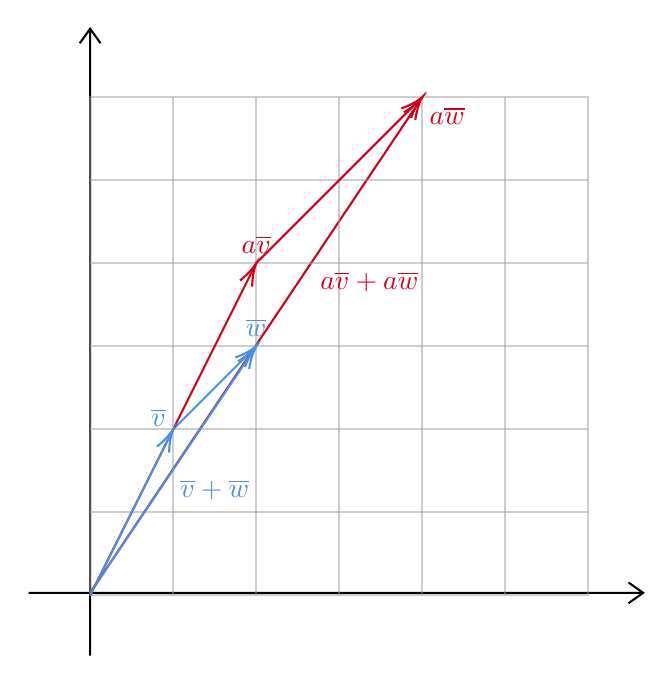
\begin{tikzpicture}[x=0.75pt,y=0.75pt,yscale=-1,xscale=1]
%uncomment if require: \path (0,423); %set diagram left start at 0, and has height of 423

%Straight Lines [id:da7905086094561125] 
\draw [color={rgb, 255:red, 208; green, 2; blue, 27 }  ,draw opacity=1 ]   (215.6,324.8) -- (374.49,87.66) ;
\draw [shift={(375.6,86)}, rotate = 123.82] [color={rgb, 255:red, 208; green, 2; blue, 27 }  ,draw opacity=1 ][line width=0.75]    (10.93,-3.29) .. controls (6.95,-1.4) and (3.31,-0.3) .. (0,0) .. controls (3.31,0.3) and (6.95,1.4) .. (10.93,3.29)   ;
%Shape: Axis 2D [id:dp7962121836036462] 
\draw  (186,324.8) -- (482,324.8)(215.6,53) -- (215.6,355) (475,319.8) -- (482,324.8) -- (475,329.8) (210.6,60) -- (215.6,53) -- (220.6,60)  ;
%Shape: Grid [id:dp7870996256892415] 
\draw  [draw opacity=0] (215.6,86) -- (455.6,86) -- (455.6,326) -- (215.6,326) -- cycle ; \draw  [color={rgb, 255:red, 155; green, 155; blue, 155 }  ,draw opacity=0.5 ] (255.6,86) -- (255.6,326)(295.6,86) -- (295.6,326)(335.6,86) -- (335.6,326)(375.6,86) -- (375.6,326)(415.6,86) -- (415.6,326) ; \draw  [color={rgb, 255:red, 155; green, 155; blue, 155 }  ,draw opacity=0.5 ] (215.6,126) -- (455.6,126)(215.6,166) -- (455.6,166)(215.6,206) -- (455.6,206)(215.6,246) -- (455.6,246)(215.6,286) -- (455.6,286) ; \draw  [color={rgb, 255:red, 155; green, 155; blue, 155 }  ,draw opacity=0.5 ] (215.6,86) -- (455.6,86) -- (455.6,326) -- (215.6,326) -- cycle ;
%Straight Lines [id:da6128088926831519] 
\draw [color={rgb, 255:red, 74; green, 144; blue, 226 }  ,draw opacity=1 ]   (255.6,246) -- (294.19,207.41) ;
\draw [shift={(295.6,206)}, rotate = 135] [color={rgb, 255:red, 74; green, 144; blue, 226 }  ,draw opacity=1 ][line width=0.75]    (10.93,-3.29) .. controls (6.95,-1.4) and (3.31,-0.3) .. (0,0) .. controls (3.31,0.3) and (6.95,1.4) .. (10.93,3.29)   ;
%Straight Lines [id:da9944692355606897] 
\draw [color={rgb, 255:red, 74; green, 144; blue, 226 }  ,draw opacity=1 ]   (215.6,324.8) -- (294.48,207.66) ;
\draw [shift={(295.6,206)}, rotate = 123.96] [color={rgb, 255:red, 74; green, 144; blue, 226 }  ,draw opacity=1 ][line width=0.75]    (10.93,-3.29) .. controls (6.95,-1.4) and (3.31,-0.3) .. (0,0) .. controls (3.31,0.3) and (6.95,1.4) .. (10.93,3.29)   ;
%Straight Lines [id:da7148545358160481] 
\draw [color={rgb, 255:red, 208; green, 2; blue, 27 }  ,draw opacity=1 ]   (215.6,326) -- (294.71,167.79) ;
\draw [shift={(295.6,166)}, rotate = 116.57] [color={rgb, 255:red, 208; green, 2; blue, 27 }  ,draw opacity=1 ][line width=0.75]    (10.93,-3.29) .. controls (6.95,-1.4) and (3.31,-0.3) .. (0,0) .. controls (3.31,0.3) and (6.95,1.4) .. (10.93,3.29)   ;
%Straight Lines [id:da27745396609468553] 
\draw [color={rgb, 255:red, 74; green, 144; blue, 226 }  ,draw opacity=1 ]   (215.6,326) -- (254.71,247.79) ;
\draw [shift={(255.6,246)}, rotate = 116.57] [color={rgb, 255:red, 74; green, 144; blue, 226 }  ,draw opacity=1 ][line width=0.75]    (10.93,-3.29) .. controls (6.95,-1.4) and (3.31,-0.3) .. (0,0) .. controls (3.31,0.3) and (6.95,1.4) .. (10.93,3.29)   ;
%Straight Lines [id:da07820003545479248] 
\draw [color={rgb, 255:red, 208; green, 2; blue, 27 }  ,draw opacity=1 ]   (295.6,166) -- (374.19,87.41) ;
\draw [shift={(375.6,86)}, rotate = 135] [color={rgb, 255:red, 208; green, 2; blue, 27 }  ,draw opacity=1 ][line width=0.75]    (10.93,-3.29) .. controls (6.95,-1.4) and (3.31,-0.3) .. (0,0) .. controls (3.31,0.3) and (6.95,1.4) .. (10.93,3.29)   ;

% Text Node
\draw (253.6,246.1) node [anchor=south east] [inner sep=0.75pt]  [color={rgb, 255:red, 74; green, 144; blue, 226 }  ,opacity=1 ]  {$\overline{v}$};
% Text Node
\draw (295.6,202.6) node [anchor=south] [inner sep=0.75pt]  [color={rgb, 255:red, 74; green, 144; blue, 226 }  ,opacity=1 ]  {$\overline{w}$};
% Text Node
\draw (257.6,268.8) node [anchor=north west][inner sep=0.75pt]  [color={rgb, 255:red, 74; green, 144; blue, 226 }  ,opacity=1 ]  {$\overline{v} +\overline{w}$};
% Text Node
\draw (295.6,162.6) node [anchor=south] [inner sep=0.75pt]  [color={rgb, 255:red, 208; green, 2; blue, 27 }  ,opacity=1 ]  {$a\overline{v}$};
% Text Node
\draw (377.6,89.4) node [anchor=north west][inner sep=0.75pt]  [color={rgb, 255:red, 208; green, 2; blue, 27 }  ,opacity=1 ]  {$a\overline{w}$};
% Text Node
\draw (325,168.73) node [anchor=north west][inner sep=0.75pt]  [color={rgb, 255:red, 208; green, 2; blue, 27 }  ,opacity=1 ]  {$a\overline{v} +a\overline{w}$};


\end{tikzpicture}
